\documentclass[10pt]{beamer}
\usetheme{metropolis}

% ── Packages ──
\usepackage{amsmath,amssymb,amsthm}
\usepackage{tikz}
\usetikzlibrary{positioning,arrows.meta,matrix,fit}
\usepackage{graphicx}
\usepackage{array}

% ── Theorem environments ──
\theoremstyle{definition}
\newtheorem{defi}{Definition}[section]
\newtheorem{prop}{Proposition}[section]
\newtheorem{cor}{Corollary}[section]

\setbeamercolor{block title}{bg=red!75!black,fg=white}
\setbeamercolor{block body}{bg=yellow!10!white}

% ── Emoji definitions ──
\newcommand{\bean}{
\includegraphics[scale=0.07]{Pictures/bean.png}}
\newcommand{\leaf}{
\includegraphics[scale=0.08]{Pictures/leaf.png}}
\newcommand{\lemon}{
\includegraphics[scale=0.08]{Pictures/lemon.png}}
\newcommand{\cow}{
\includegraphics[scale=0.08]{Pictures/cow.png}}
\newcommand{\milk}{
\includegraphics[scale=0.07]{Pictures/milk.png}}
\newcommand{\coffee}{
\includegraphics[scale=0.10]{Pictures/coffee.png}}
\newcommand{\tea}{
\includegraphics[scale=0.08]{Pictures/tea.png}}
\newcommand{\bento}{
\includegraphics[scale=0.09]{Pictures/bento.png}}
\newcommand{\ramen}{
\includegraphics[scale=0.09]{Pictures/soup.png}}

% ── Cross-filling color commands ──
\newcommand{\pvt}[1]{{\color{red}\mathbf{#1}}}       % pivot
\newcommand{\crs}[1]{{\color{blue}#1}}                % cross arm
\newcommand{\rem}[1]{{\color{gray}#1}}                % remainder zero

% ── Highlighting ──
\newcommand{\x}[1]{\alert{\textbf{#1}}}

\title{Cross-Filling Method}
\subtitle{Finding Hidden Patterns in Recipe Tables}
\date{}

\begin{document}

\maketitle

% ═══════════════════════════════════════
% §0 INTRODUCTION
% ═══════════════════════════════════════
\section{Introduction}

\begin{frame}{Learning Objectives}
Logic maps for today's cross-filling method's place in the big picture:
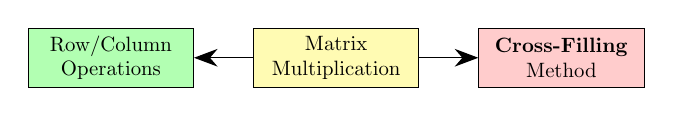
\begin{tikzpicture}[scale=0.75,transform shape,
    block/.style={draw, rectangle, minimum width=2.8cm, minimum height=1cm, align=center}]
\node[block,fill=green!30] (block1) {Row/Column\\Operations};
\node[block, right=1cm of block1, fill=yellow!30] (block2) {Matrix\\Multiplication};
\node[block, right=1cm of block2, fill=red!20] (block3) {\textbf{Cross-Filling}\\Method};
\draw[-{Stealth[length=3mm]}] (block2) -- (block1);
\draw[-{Stealth[length=3mm]}] (block2) -- (block3);
\end{tikzpicture}

\vspace{0.5cm}
\textbf{Key Questions:}
\begin{itemize}
\item Can we \x{discover hidden intermediate products} from a direct recipe table?
\item What is a \x{simple pattern} (rank-one table)?
\item How to \x{decompose} complex tables into simple patterns?
\item How to convert between \x{sum} and \x{product} forms?
\end{itemize}
\end{frame}

\begin{frame}{Review: Sum-of-Rank-One View}
Recall from Lecture 1, matrix multiplication $C = AB$ has three views:

$$C =
\begin{pmatrix}
| & | & & | \\
a_1 & a_2 & \cdots & a_n \\
| & | & & |
\end{pmatrix}
\begin{pmatrix}
- & b_1^T & - \\
- & b_2^T & - \\
\vdots & \vdots & \vdots \\
- & b_n^T & -
\end{pmatrix}
= \sum_{k=1}^{n} a_k \, b_k^T$$

\vfill
Each $a_k \, b_k^T$ is called a \x{rank-one piece} (column $\times$ row).

\vfill
\textbf{Today's question}: Can we \x{reverse} this? Given $C$, find the pieces?
\end{frame}

% ═══════════════════════════════════════
% §1 CONCRETIZATION PHASE: DISCOVERING PATTERNS
% ═══════════════════════════════════════
\section{Discovering Simple Patterns (Concretization)}

\begin{frame}{The Motivating Problem}
\textbf{Coffee shop scenario:}

We have a \x{direct} recipe table from raw materials to final products:
$$C = \begin{array}{c|cc}
 & \text{\bento} & \text{\ramen} \\
\hline
\text{\leaf} & 2 & 2 \\
\text{\lemon} & 1 & 1 \\
\text{\bean} & 0 & 4 \\
\text{\cow} & 2 & 1
\end{array}$$

\vfill
\textbf{Question}: Are there \x{hidden intermediate products} (like \milk, \coffee, \tea) that we could use to simplify this?
\end{frame}

\begin{frame}{What is a Simple Pattern?}
Look at the first two rows of our table:
$$\begin{array}{c|cc}
 & \text{\bento} & \text{\ramen} \\
\hline
\text{\leaf} & 2 & 2 \\
\text{\lemon} & 1 & 1
\end{array}$$

\vfill
\textbf{Notice}: Both products use \x{the same amount}!
\begin{itemize}
\item \bento: 2\leaf~+ 1\lemon
\item \ramen: 2\leaf~+ 1\lemon
\end{itemize}

\vfill
Can we extract this \x{common base} and see what's different?
\end{frame}

\begin{frame}{Setup: The Full Direct Table}
$$C = \begin{array}{c|cc}
 & \text{\bento} & \text{\ramen} \\
\hline
\text{\leaf} & 2 & 2 \\
\text{\lemon} & 1 & 1 \\
\text{\bean} & 0 & 4 \\
\text{\cow} & 2 & 1
\end{array}$$

\vfill
We noticed: first two rows have the same pattern.

\vfill
Can we \x{extract} this pattern and see what's left?
\end{frame}

\begin{frame}{Change: Choose a Pivot}
\textbf{Pick a pivot} (center of our cross):

Let's pick the \leaf~row and \bento~column. Entry = 2.

$$C = \begin{array}{c|cc}
 & \text{\bento} & \text{\ramen} \\
\hline
\text{\leaf} & \pvt{2} & 2 \\
\text{\lemon} & 1 & 1 \\
\text{\bean} & 0 & 4 \\
\text{\cow} & 2 & 1
\end{array}$$

\vfill
This pivot will be the \x{center of our cross}.
\end{frame}

\begin{frame}{Calculation Step 1: Extract the Cross}
The \x{cross} through the pivot includes:
\begin{itemize}
\item Entire \leaf~row (row through pivot)
\item Entire \bento~column (column through pivot)
\end{itemize}

$$C = \begin{array}{c|cc}
 & \text{\bento} & \text{\ramen} \\
\hline
\text{\leaf} & \pvt{2} & \crs{2} \\
\text{\lemon} & \crs{1} & 1 \\
\text{\bean} & \crs{0} & 4 \\
\text{\cow} & \crs{2} & 1
\end{array}$$

\vfill
Cross row: $(2, 2)$ \quad Cross column: $(2, 1, 0, 2)$
\end{frame}

\begin{frame}{Calculation Step 2: Build the Pattern Table}
\textbf{Idea}: Use the cross to fill all entries via "multiplication table":

$$\text{New entry} = \frac{\text{(column value)} \times \text{(row value)}}{\text{pivot}}$$

\vfill
For \ramen~and \lemon:
$$\text{Entry} = \frac{\crs{1} \times \crs{2}}{\pvt{2}} = 1$$

For \ramen~and \bean:
$$\text{Entry} = \frac{\crs{0} \times \crs{2}}{\pvt{2}} = 0$$
\end{frame}

\begin{frame}{Result: The First Pattern $R_1$}
$$R_1 = \begin{array}{c|cc}
 & \text{\bento} & \text{\ramen} \\
\hline
\text{\leaf} & \pvt{2} & \crs{2} \\
\text{\lemon} & \crs{1} & 1 \\
\text{\bean} & \crs{0} & 0 \\
\text{\cow} & \crs{2} & 2
\end{array}$$

\vfill
\textbf{Interpretation}: This is the \x{common base recipe}!
\begin{itemize}
\item Base recipe: 2\leaf~+ 1\lemon~+ 0\bean~+ 2\cow
\item \bento~uses: 1× base
\item \ramen~uses: 1× base (+ adjustments)
\end{itemize}
\end{frame}

\begin{frame}{Insight: What is This Pattern?}
The pattern $R_1$ is a \x{rank-one matrix}:

$$R_1 = \begin{pmatrix} 2 \\ 1 \\ 0 \\ 2 \end{pmatrix}
\begin{pmatrix} 1 & 1 \end{pmatrix}$$

\vspace{0.3cm}
- \x{Column} $(2,1,0,2)$: the base recipe
- \x{Row} $(1,1)$: both products use 1× this base

\vspace{0.3cm}
Key: \x{One pattern, repeated!} Both columns are the same.
\end{frame}

\begin{frame}{Setup: What's Left After $R_1$?}
Subtract $R_1$ from the original table $C$:

$$C - R_1 = \begin{array}{c|cc}
 & \text{\bento} & \text{\ramen} \\
\hline
\text{\leaf} & 2-2 & 2-2 \\
\text{\lemon} & 1-1 & 1-1 \\
\text{\bean} & 0-0 & 4-0 \\
\text{\cow} & 2-2 & 1-2
\end{array}$$
\end{frame}

\begin{frame}{Result: The Remainder}
$$C_2 = C - R_1 = \begin{array}{c|cc}
 & \text{\bento} & \text{\ramen} \\
\hline
\text{\leaf} & \rem{0} & \rem{0} \\
\text{\lemon} & \rem{0} & \rem{0} \\
\text{\bean} & \rem{0} & 4 \\
\text{\cow} & \rem{0} & -1
\end{array}$$

\vfill
\textbf{What's left?}
- \bento~column: all zeros (base recipe exactly matches!)
- \ramen~column: adjustments needed (+4\bean, -1\cow)
\end{frame}

\begin{frame}{Insight: Why "Cross-Filling"?}
\begin{center}
\begin{tikzpicture}[scale=0.6, every node/.style={scale=0.85}]
% Original
\node at (0,4) {\small Original};
\node at (0,1.5) {$\begin{array}{c|cc}
\text{\leaf} & 2 & 2 \\
\text{\lemon} & 1 & 1 \\
\text{\bean} & 0 & 4 \\
\text{\cow} & 2 & 1
\end{array}$};

% Arrow
\draw[-{Stealth},thick] (1.8,1.5) -- (3,1.5);
\node at (2.4,2) {\tiny pick pivot};

% Cross
\node at (5,4) {\small Extract \x{cross}};
\node at (5,1.5) {$\begin{array}{c|cc}
\text{\leaf} & \pvt{2} & \crs{2} \\
\text{\lemon} & \crs{1} & \cdot \\
\text{\bean} & \crs{0} & \cdot \\
\text{\cow} & \crs{2} & \cdot
\end{array}$};

% Arrow
\draw[-{Stealth},thick] (6.8,1.5) -- (8,1.5);
\node at (7.4,2) {\tiny fill};

% Filled
\node at (10,4) {\small \x{Fill} pattern};
\node at (10,1.5) {$\begin{array}{c|cc}
\text{\leaf} & \pvt{2} & \crs{2} \\
\text{\lemon} & \crs{1} & 1 \\
\text{\bean} & \crs{0} & 0 \\
\text{\cow} & \crs{2} & 2
\end{array}$};

% Arrow
\draw[-{Stealth},thick] (11.8,1.5) -- (13,1.5);
\node at (12.4,2) {\tiny subtract};

% Remainder
\node at (15,4) {\small Remainder};
\node at (15,1.5) {$\begin{array}{c|cc}
\text{\leaf} & \rem{0} & \rem{0} \\
\text{\lemon} & \rem{0} & \rem{0} \\
\text{\bean} & \rem{0} & 4 \\
\text{\cow} & \rem{0} & -1
\end{array}$};
\end{tikzpicture}
\end{center}

\vfill
The method \x{fills in} the cross region, then eliminates it!
\end{frame}

\begin{frame}{Change: Find Second Pattern}
Look at the remainder:
$$C_2 = \begin{array}{c|cc}
 & \text{\bento} & \text{\ramen} \\
\hline
\text{\bean} & 0 & 4 \\
\text{\cow} & 0 & -1
\end{array}$$

\vfill
This is the \x{adjustment} for \ramen: +4\bean, -1\cow

\vfill
Pick pivot: \bean~row, \ramen~column. Entry = 4.
\end{frame}

\begin{frame}{Calculation: Fill Second Cross}
Pivot at (3,2) = 4. Cross: column $(0,0,4,-1)^T$, row $(0,4)$

$$R_2 = \frac{1}{\pvt{4}}
\begin{pmatrix} 0 \\ 0 \\ 4 \\ -1 \end{pmatrix}
\begin{pmatrix} 0 & 4 \end{pmatrix}
= \begin{array}{c|cc}
 & \text{\bento} & \text{\ramen} \\
\hline
\text{\leaf} & 0 & 0 \\
\text{\lemon} & 0 & 0 \\
\text{\bean} & 0 & \pvt{4} \\
\text{\cow} & 0 & -1
\end{array}$$

\vfill
\textbf{Interpretation}: The \x{adjustment term} — only affects \ramen.
\end{frame}

\begin{frame}{Result: Complete Decomposition}
$$C_2 - R_2 = \begin{array}{c|cc}
 & \text{\bento} & \text{\ramen} \\
\hline
\text{\bean} & 0 & 0 \\
\text{\cow} & 0 & 0
\end{array}$$

\vfill
\x{Done!} Remainder is zero.
\end{frame}

\begin{frame}{The Full Decomposition}
\textbf{We discovered:}
$$C = R_1 + R_2$$

$$\begin{array}{c|cc}
\text{\leaf} & 2 & 2 \\
\text{\lemon} & 1 & 1 \\
\text{\bean} & 0 & 4 \\
\text{\cow} & 2 & 1
\end{array}
=
\begin{array}{c|cc}
\text{\leaf} & 2 & 2 \\
\text{\lemon} & 1 & 1 \\
\text{\bean} & 0 & 0 \\
\text{\cow} & 2 & 2
\end{array}
+
\begin{array}{c|cc}
\text{\leaf} & 0 & 0 \\
\text{\lemon} & 0 & 0 \\
\text{\bean} & 0 & 4 \\
\text{\cow} & 0 & -1
\end{array}$$

\vfill
Two \x{rank-one patterns}: base recipe + adjustment!
\end{frame}

\begin{frame}{Insight: Base + Adjustment Decomposition}
\textbf{What we found:}

$$\text{\ramen} = 1 \times (\text{base recipe}) + \text{adjustment}$$

\vfill
Key insight:
\begin{itemize}
\item $R_1$: Common base shared by both products
\item $R_2$: Adjustment term (only for \ramen)
\item \bento~= exactly the base recipe
\item \ramen~= base + extra 4\bean~- 1\cow
\end{itemize}

\vfill
This is \x{expressing complex recipes in terms of simpler patterns}!
\end{frame}

% ═══════════════════════════════════════
% §2 CHANGE OF PERSPECTIVE
% ═══════════════════════════════════════
\section{Change of Perspective}

\begin{frame}{Change of Perspective}
\textbf{What we've learned so far:}
\begin{itemize}
\item \x{What} a simple pattern (rank-one) looks like — one base mix used in different amounts
\item \x{How} to extract patterns using cross-filling — pick pivot, fill cross, subtract
\item \x{Why} this works — discovers hidden intermediate products
\end{itemize}

\vspace{0.5cm}
\begin{alertblock}{From This Point Forward}
We \x{forget about coffee shops} and work with \x{abstract matrices}:
\begin{itemize}
\item \textbf{What}: Matrices $A$, $B$, $C$, rank-one pieces $R_k$
\item \textbf{How}: Cross-filling algorithm, sum $\leftrightarrow$ product conversion
\item \textbf{Why}: Compute rank, factorizations, solve equations
\end{itemize}
\end{alertblock}

\vspace{0.3cm}
This simplifies notation while preserving the intuition.
\end{frame}

% ═══════════════════════════════════════
% §3 FORMALIZATION PHASE: DEFINITIONS AND ALGORITHMS
% ═══════════════════════════════════════
\section{Rank-One Matrices (Formalization)}

\begin{frame}{Definition: Rank-One Matrix}
\begin{defi}[Rank-One Matrix]
A matrix $R$ is \x{rank-one} if it can be written as
$$R = \mathbf{u}\, \mathbf{v}^T$$
for some nonzero column vector $\mathbf{u}$ and nonzero row vector $\mathbf{v}^T$.
\end{defi}

\vspace{0.3cm}
Example:
$$R = \begin{pmatrix} 2 \\ 1 \\ 3 \end{pmatrix} \begin{pmatrix} 1 & 2 \end{pmatrix}
= \begin{pmatrix}
2 & 4 \\
1 & 2 \\
3 & 6
\end{pmatrix}$$

\vspace{0.2cm}
Key: All columns are multiples of $\mathbf{u}$. All rows are multiples of $\mathbf{v}^T$.
\end{frame}

\begin{frame}{Recognizing Rank-One Structure}
Is this matrix rank-one?
$$\begin{pmatrix}
6 & 9 & 3 \\
4 & 6 & 2 \\
10 & 15 & 5
\end{pmatrix}$$

\vfill
Check rows:
\begin{itemize}
\item Row 1: $(6, 9, 3) = 3 \cdot (2, 3, 1)$
\item Row 2: $(4, 6, 2) = 2 \cdot (2, 3, 1)$
\item Row 3: $(10, 15, 5) = 5 \cdot (2, 3, 1)$
\end{itemize}

\vfill
Yes!\ \ $R = \begin{pmatrix} 3 \\ 2 \\ 5 \end{pmatrix} \begin{pmatrix} 2 & 3 & 1 \end{pmatrix}$
\end{frame}

\begin{frame}[fragile]{Cross-Product Property}
In a rank-one matrix $R = \mathbf{u}\,\mathbf{v}^T$, every entry is $r_{ij} = u_i v_j$.

\vfill
\textbf{Visual meaning of subscripts:}

\begin{center}
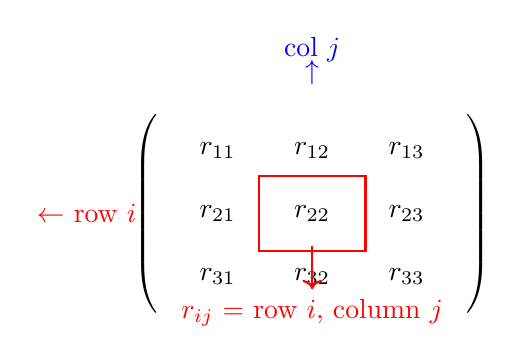
\begin{tikzpicture}[scale=0.8]
% Matrix with labeled positions
\matrix (m) [matrix of math nodes, left delimiter=(, right delimiter=),
             nodes={minimum width=1.2cm, minimum height=0.8cm}] {
  r_{11} & r_{12} & r_{13} \\
  r_{21} & r_{22} & r_{23} \\
  r_{31} & r_{32} & r_{33} \\
};
% Highlight r_{ij}
\node[draw=red, thick, fit=(m-2-2), inner sep=2pt] {};
\draw[->,red,thick] (m-2-2) -- ++(0,-1.2) node[below] {$r_{ij}$ = row $i$, column $j$};
% Label rows and columns
\node[left=0.3cm of m-2-1, red] {$\leftarrow$ row $i$};
\node[above=0.3cm of m-1-2, blue] {$\uparrow$};
\node[above=0.6cm of m-1-2, blue] {col $j$};
\end{tikzpicture}
\end{center}

\vfill

\end{frame}
\begin{frame}[fragile]{Cross-Product Property}
%\end{frame}
%\begin{frame}{}
For any four entries forming a rectangle:
$$\boxed{r_{ij} \cdot r_{k\ell} = r_{i\ell} \cdot r_{kj}}$$

\begin{center}
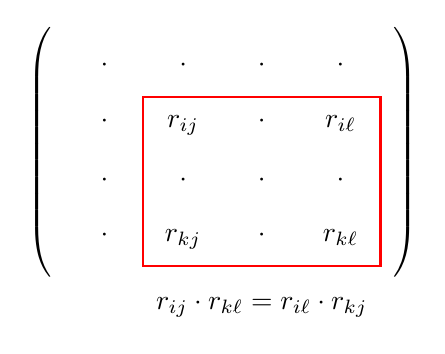
\begin{tikzpicture}[scale=0.7]
\matrix (m) [matrix of math nodes, left delimiter=(, right delimiter=),
             nodes={minimum width=1cm, minimum height=0.7cm}] {
  \cdot & \cdot & \cdot & \cdot \\
  \cdot & r_{ij} & \cdot & r_{i\ell} \\
  \cdot & \cdot & \cdot & \cdot \\
  \cdot & r_{kj} & \cdot & r_{k\ell} \\
};
\draw[red,thick] (m-2-2.north west) rectangle (m-4-4.south east);
\node[below=0.3cm of m-4-3] {$r_{ij} \cdot r_{k\ell} = r_{i\ell} \cdot r_{kj}$};
\end{tikzpicture}
\end{center}

\textbf{Why?}\ \ $(u_i v_j)(u_k v_\ell) = (u_i v_\ell)(u_k v_j) = u_i u_k v_j v_\ell$
\end{frame}

\begin{frame}{Not Every Matrix is Rank-One}
$$C = \begin{pmatrix}
2 & 4 \\
1 & 2 \\
3 & 7
\end{pmatrix}$$

\vfill
Check ratios: $\frac{4}{2} = 2$, \quad $\frac{2}{1} = 2$, \quad $\frac{7}{3} \neq 2$ \quad $\leftarrow$ Different!

\vfill
This is \x{not rank-one}. But can we write it as a \x{sum} of rank-one pieces?

$$C = \underbrace{\begin{pmatrix} ? \end{pmatrix}}_{R_1} + \underbrace{\begin{pmatrix} ? \end{pmatrix}}_{R_2} + \cdots$$

Cross-filling answers this!
\end{frame}

% ═══════════════════════════════════════
% §4 CROSS-FILLING ALGORITHM
% ═══════════════════════════════════════
\section{Cross-Filling Algorithm}

\begin{frame}[fragile]{The Cross-Filling Algorithm}
\begin{prop}[Cross-Filling Algorithm]
\textbf{Input}: Matrix $A$ ($m \times n$)

\textbf{Output}: $A = R_1 + R_2 + \cdots + R_r$ (sum of rank-one matrices)

\textbf{Procedure}:
\begin{enumerate}
\item Find any nonzero entry $a_{ij} \neq 0$ (the \x{pivot})

\hspace{1cm}
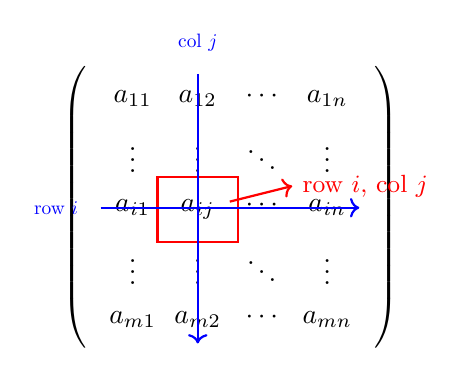
\begin{tikzpicture}[scale=0.6,baseline=(current bounding box.center)]
\matrix (m) [matrix of math nodes, left delimiter=(, right delimiter=),
             nodes={minimum width=0.8cm, minimum height=0.6cm}] {
  a_{11} & a_{12} & \cdots & a_{1n} \\
  \vdots & \vdots & \ddots & \vdots \\
  a_{i1} & a_{ij} & \cdots & a_{in} \\
  \vdots & \vdots & \ddots & \vdots \\
  a_{m1} & a_{m2} & \cdots & a_{mn} \\
};
\node[draw=red, thick, fit=(m-3-2), inner sep=3pt] {};
\draw[->,red,thick] (m-3-2) -- ++(2,0.5) node[right] {\small row $i$, col $j$};
\draw[->,blue,thick] (m-3-1.west) -- (m-3-4.east);
\draw[->,blue,thick] (m-1-2.north) -- (m-5-2.south);
\node[left=0.2cm of m-3-1, blue, scale=0.7] {row $i$};
\node[above=0.2cm of m-1-2, blue, scale=0.7] {col $j$};
\end{tikzpicture}
\end{enumerate}
\end{prop}
\end{frame}
\begin{frame}[fragile]{Cross-Filling Algorithm (continued)}
\begin{prop}[Cross-Filling Algorithm (continued)]
\begin{enumerate}
\item Extract the cross: row $i$ and column $j$
\item Form rank-one piece:
$$R = \frac{1}{a_{ij}} \cdot (\text{column } j) \cdot (\text{row } i)$$
\item Compute remainder: $A' = A - R$
\item Repeat on $A'$ until $A' = O$
\end{enumerate}
\end{prop}

\vspace{0.2cm}
Each step eliminates one cross (one row and one column become zero).
\end{frame}

\begin{frame}{Pivot Selection Principles}
\textbf{Key Question}: Which nonzero entry should we pick as pivot?

\vfill
\begin{alertblock}{Pivot Independence Principle}
At each step, choose any nonzero entry $a_{ij} \neq 0$ such that:
\begin{itemize}
\item Row $i$ is \x{not yet zeroed} by previous steps
\item Column $j$ is \x{not yet zeroed} by previous steps
\end{itemize}
\end{alertblock}


\vfill
\textbf{Consequence}: \x{Many different pivot sequences are valid!}
\begin{itemize}
\item Diagonal pivots $(1,1) \to (2,2) \to \cdots$ ← one choice
\item Off-diagonal pivots $(1,3) \to (2,1) \to \cdots$ ← also valid!
\item Different sequences give different decompositions, but \x{same rank}
\end{itemize}
\end{frame}

\begin{frame}{Example: Diagonal Cross-Filling}
Decompose using diagonal pivots:
$$A = \begin{pmatrix}
1 & 1 & 1 \\
1 & 3 & 3 \\
1 & 3 & 8
\end{pmatrix}$$

\vfill
Strategy: Pick pivots $(1,1) \to (2,2) \to (3,3)$

\vfill
We will see this produces \x{LU decomposition} structure.
\end{frame}

\begin{frame}[fragile]{Iteration 1: Pivot $a_{11} = 1$}

\textbf{Choosing position $(1,1)$:}

\begin{center}
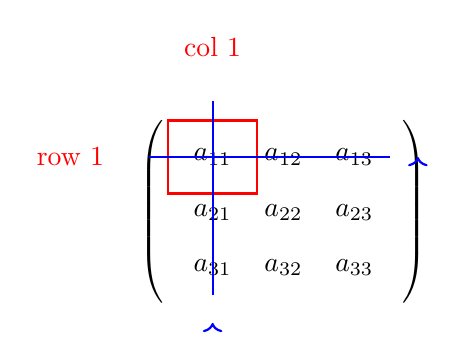
\begin{tikzpicture}[scale=0.7]
\matrix (m) [matrix of math nodes, left delimiter=(, right delimiter=),
             nodes={minimum width=0.9cm, minimum height=0.7cm}] {
  a_{11} & a_{12} & a_{13} \\
  a_{21} & a_{22} & a_{23} \\
  a_{31} & a_{32} & a_{33} \\
};
\node[draw=red, thick, fit=(m-1-1), inner sep=3pt] {};
\draw[->,blue,thick] (m-1-1.west) ++ (-0.5,0) -- (m-1-3.east) ++ (0.5,0);
\draw[->,blue,thick] (m-1-1.north) ++ (0,0.5) -- (m-3-1.south) ++ (0,-0.5);
\node[left=0.8cm of m-1-1, red] {row 1};
\node[above=0.8cm of m-1-1, red] {col 1};
\end{tikzpicture}
\end{center}

Highlight the cross:
$$A = \begin{pmatrix}
\pvt{1} & \crs{1} & \crs{1} \\
\crs{1} & 3 & 3 \\
\crs{1} & 3 & 8
\end{pmatrix}$$
\end{frame}
\begin{frame}[fragile]{Iteration 1: Fill the Cross}

Fill using the cross:
$$R_1 = \frac{1}{\pvt{1}}
\begin{pmatrix} \crs{1} \\ \crs{1} \\ \crs{1} \end{pmatrix}
\begin{pmatrix} \crs{1} & \crs{1} & \crs{1} \end{pmatrix}
= \begin{pmatrix}
\pvt{1} & \crs{1} & \crs{1} \\
\crs{1} & 1 & 1 \\
\crs{1} & 1 & 1
\end{pmatrix}$$
\end{frame}

\begin{frame}{Iteration 1: Remainder $A_1$}
$$A_1 = A - R_1 = \begin{pmatrix}
1 & 1 & 1 \\
1 & 3 & 3 \\
1 & 3 & 8
\end{pmatrix}
- \begin{pmatrix}
1 & 1 & 1 \\
1 & 1 & 1 \\
1 & 1 & 1
\end{pmatrix}
= \begin{pmatrix}
\rem{0} & \rem{0} & \rem{0} \\
\rem{0} & 2 & 2 \\
\rem{0} & 2 & 7
\end{pmatrix}$$

\vfill
Row 1 and column 1 are now \rem{zero}.\ \ $\checkmark$
\end{frame}

\begin{frame}[fragile]{Iteration 2: Pivot $(A_1)_{22} = 2$}

\textbf{Choosing position $(2,2)$ in the remainder:}

\begin{center}
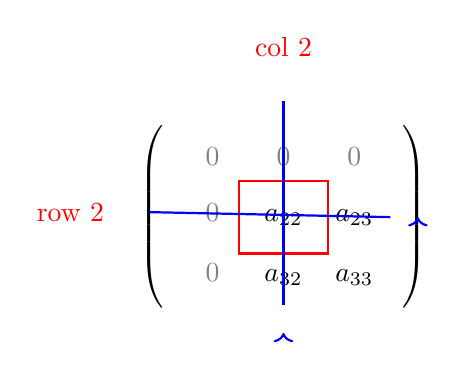
\begin{tikzpicture}[scale=0.7]
\matrix (m) [matrix of math nodes, left delimiter=(, right delimiter=),
             nodes={minimum width=0.9cm, minimum height=0.7cm}] {
  \rem{0} & \rem{0} & \rem{0} \\
  \rem{0} & a_{22} & a_{23} \\
  \rem{0} & a_{32} & a_{33} \\
};
\node[draw=red, thick, fit=(m-2-2), inner sep=3pt] {};
\draw[->,blue,thick] (m-2-1.west) ++ (-0.5,0) -- (m-2-3.east) ++ (0.5,0);
\draw[->,blue,thick] (m-1-2.north) ++ (0,0.5) -- (m-3-2.south) ++ (0,-0.5);
\node[left=0.8cm of m-2-1, red] {row 2};
\node[above=0.8cm of m-1-2, red] {col 2};
\end{tikzpicture}
\end{center}

$$A_1 = \begin{pmatrix}
\rem{0} & \rem{0} & \rem{0} \\
\rem{0} & \pvt{2} & \crs{2} \\
\rem{0} & \crs{2} & 7
\end{pmatrix}$$

\end{frame}
\begin{frame}[fragile]{Iteration 2: Fill the Cross}
Fill:
$$R_2 = \frac{1}{\pvt{2}}
\begin{pmatrix} \rem{0} \\ \crs{2} \\ \crs{2} \end{pmatrix}
\begin{pmatrix} \rem{0} & \crs{2} & \crs{2} \end{pmatrix}
= \begin{pmatrix}
\rem{0} & \rem{0} & \rem{0} \\
\rem{0} & \pvt{2} & \crs{2} \\
\rem{0} & \crs{2} & 2
\end{pmatrix}$$
\end{frame}

\begin{frame}{Iteration 2: Remainder $A_2$}
$$A_2 = A_1 - R_2 = \begin{pmatrix}
0 & 0 & 0 \\
0 & 2 & 2 \\
0 & 2 & 7
\end{pmatrix}
- \begin{pmatrix}
0 & 0 & 0 \\
0 & 2 & 2 \\
0 & 2 & 2
\end{pmatrix}
= \begin{pmatrix}
\rem{0} & \rem{0} & \rem{0} \\
\rem{0} & \rem{0} & \rem{0} \\
\rem{0} & \rem{0} & 5
\end{pmatrix}$$

\vfill
Rows 1--2 and columns 1--2 are now \rem{zero}.\ \ $\checkmark$
\end{frame}

\begin{frame}{Iteration 3: Final Piece}
$$A_2 = \begin{pmatrix}
\rem{0} & \rem{0} & \rem{0} \\
\rem{0} & \rem{0} & \rem{0} \\
\rem{0} & \rem{0} & \pvt{5}
\end{pmatrix}$$

\vfill
This is already rank-one:
$$R_3 = \begin{pmatrix} 0 \\ 0 \\ 1 \end{pmatrix}
\begin{pmatrix} 0 & 0 & 5 \end{pmatrix}
= \begin{pmatrix}
\rem{0} & \rem{0} & \rem{0} \\
\rem{0} & \rem{0} & \rem{0} \\
\rem{0} & \rem{0} & \pvt{5}
\end{pmatrix}$$

Remainder: $A_3 = A_2 - R_3 = O$. \quad \x{Done!}
\end{frame}

\begin{frame}{Full Decomposition (Diagonal Pivots)}
$$A = \underbrace{\begin{pmatrix}
\pvt{1} & \crs{1} & \crs{1} \\
\crs{1} & 1 & 1 \\
\crs{1} & 1 & 1
\end{pmatrix}}_{R_1}
+ \underbrace{\begin{pmatrix}
\rem{0} & \rem{0} & \rem{0} \\
\rem{0} & \pvt{2} & \crs{2} \\
\rem{0} & \crs{2} & 2
\end{pmatrix}}_{R_2}
+ \underbrace{\begin{pmatrix}
\rem{0} & \rem{0} & \rem{0} \\
\rem{0} & \rem{0} & \rem{0} \\
\rem{0} & \rem{0} & \pvt{5}
\end{pmatrix}}_{R_3}$$

\vfill
Three rank-one pieces:
\begin{itemize}
\item $R_1$: pivot $\pvt{1}$ at position $(1,1)$
\item $R_2$: pivot $\pvt{2}$ at position $(2,2)$
\item $R_3$: pivot $\pvt{5}$ at position $(3,3)$
\end{itemize}

\vfill
Key: \x{Diagonal} pivot strategy $\to$ special structure (LU decomposition)
\end{frame}

\begin{frame}{Example: Non-Diagonal Cross-Filling (Setup)}
Now let's decompose the \x{same matrix} using \x{off-diagonal pivots}:
$$A = \begin{pmatrix}
1 & 1 & 1 \\
1 & 3 & 3 \\
1 & 3 & 8
\end{pmatrix}$$

\vfill
New strategy: Pick pivots $(1,3) \to (2,1) \to (3,2)$ (all off-diagonal!)

\vfill
\textbf{Question}: Will we get a different decomposition?

\vfill
\textbf{Answer}: Yes! Different $R_k$ pieces, but \x{same rank} (still 3 pieces).
\end{frame}

\begin{frame}{Non-Diagonal Iteration 1: Pivot $(1,3)$}
Choose position $(1,3)$: entry = $1$

$$A = \begin{pmatrix}
\crs1 & \crs1 & \pvt{1} \\
1 & 3 & \crs{3} \\
1 & 3 & \crs{8}
\end{pmatrix}
\quad
\text{Cross: row 1 = $(\crs{1}, \crs{1}, \pvt{1})$, col 3 = $(\pvt{1}, \crs{3}, \crs{8})^T$}
$$

\vfill
Fill:
$$R_1' = \frac{1}{\pvt{1}}
\begin{pmatrix} \pvt{1} \\ \crs{3} \\ \crs{8} \end{pmatrix}
\begin{pmatrix} \crs{1} & \crs{1} & \pvt{1} \end{pmatrix}
= \begin{pmatrix}
\pvt{1} & \crs{1} & \crs{1} \\
3 & 3 & \crs3 \\
{8} & 8 & \crs8
\end{pmatrix}$$

\vfill
Remainder:
$$A_1' = A - R_1' = \begin{pmatrix}
\rem{0} & \rem{0} & \rem{0} \\
-2 & 0 & \rem{0} \\
-7 & -5 & \rem{0}
\end{pmatrix}$$

Row 1 and column 3 are \rem{zero}.\ \ $\checkmark$
\end{frame}

\begin{frame}{Non-Diagonal Iteration 2: Pivot $(2,1)$}
Choose position $(2,1)$ in $A_1'$: entry = $-2$

$$A_1' = \begin{pmatrix}
\rem{0} & \rem{0} & \rem{0} \\
\pvt{-2} & \crs{0} & \rem{0} \\
\crs{-7} & -5 & \rem{0}
\end{pmatrix}$$

\vfill
Fill:
$$R_2' = \frac{1}{\pvt{-2}}
\begin{pmatrix} \rem{0} \\ \pvt{-2} \\ \crs{-7} \end{pmatrix}
\begin{pmatrix} \pvt{-2} & \crs{0} & \rem{0} \end{pmatrix}
= \begin{pmatrix}
\rem{0} & \rem{0} & \rem{0} \\
\pvt{-2} & \crs{0} & \rem{0} \\
\crs{-7} & 0 & \rem{0}
\end{pmatrix}$$

\vfill
Remainder:
$$A_2' = A_1' - R_2' = \begin{pmatrix}
\rem{0} & \rem{0} & \rem{0} \\
\rem{0} & \rem{0} & \rem{0} \\
\rem{0} & -5 & \rem{0}
\end{pmatrix}$$
\end{frame}

\begin{frame}{Non-Diagonal Iteration 3: Final Piece}
$$A_2' = \begin{pmatrix}
\rem{0} & \rem{0} & \rem{0} \\
\rem{0} & \rem{0} & \rem{0} \\
\rem{0} & \pvt{-5} & \rem{0}
\end{pmatrix}$$

\vfill
$$R_3' = \begin{pmatrix} 0 \\ 0 \\ 1 \end{pmatrix}
\begin{pmatrix} 0 & -5 & 0 \end{pmatrix}
= \begin{pmatrix}
\rem{0} & \rem{0} & \rem{0} \\
\rem{0} & \rem{0} & \rem{0} \\
\rem{0} & \pvt{-5} & \rem{0}
\end{pmatrix}$$

\x{Done!}\ \ $A = R_1' + R_2' + R_3'$
\end{frame}

\begin{frame}{Comparison: Diagonal vs Non-Diagonal}
\textbf{Same matrix $A$, different pivot strategies:}

\vspace{0.3cm}
\begin{tabular}{l|c|c}
& \textbf{Diagonal} $(1,1) \to (2,2) \to (3,3)$ & \textbf{Off-diagonal} $(1,3) \to (2,1) \to (3,2)$ \\
\hline
$R_1$ & $\begin{pmatrix}
1 & 1 & 1 \\
1 & 1 & 1 \\
1 & 1 & 1
\end{pmatrix}$ &
$\begin{pmatrix}
1 & 1 & 1 \\
3 & 3 & 3 \\
8 & 8 & 8
\end{pmatrix}$ \\[10pt]
$R_2$ & $\begin{pmatrix}
0 & 0 & 0 \\
0 & 2 & 2 \\
0 & 2 & 2
\end{pmatrix}$ &
$\begin{pmatrix}
0 & 0 & 0 \\
-2 & 0 & 0 \\
-7 & 0 & 0
\end{pmatrix}$ \\[10pt]
$R_3$ & $\begin{pmatrix}
0 & 0 & 0 \\
0 & 0 & 0 \\
0 & 0 & 5
\end{pmatrix}$ &
$\begin{pmatrix}
0 & 0 & 0 \\
0 & 0 & 0 \\
0 & -5 & 0
\end{pmatrix}$ \\
\hline
\textbf{Rank} & \x{3} & \x{3} \\
\end{tabular}

\vfill
\textbf{Key}: \x{Different decompositions, same rank!}
\end{frame}

\begin{frame}{Another Example: $3 \times 4$ Matrix}
Decompose with non-diagonal pivots:
$$B = \begin{pmatrix}
2 & 0 & 4 & 2 \\
1 & 3 & 5 & 4 \\
0 & 6 & 2 & 5
\end{pmatrix}$$

\vfill
Strategy: $(2,3) \to (1,1) \to (3,2)$

\vfill
\textbf{Step 1}: Pivot at $(2,3)$, entry = $5$

Cross: row 2 = $(1, 3, 5, 4)$, col 3 = $(4, 5, 2)^T$

$$R_1 = \frac{1}{5} \begin{pmatrix} 4 \\ 5 \\ 2 \end{pmatrix}
\begin{pmatrix} 1 & 3 & 5 & 4 \end{pmatrix}
= \begin{pmatrix}
4/5 & 12/5 & 4 & 16/5 \\
1 & 3 & 5 & 4 \\
2/5 & 6/5 & 2 & 8/5
\end{pmatrix}$$
\end{frame}

\begin{frame}{$3 \times 4$ Remainder After Step 1}
$$B_1 = B - R_1 = \begin{pmatrix}
6/5 & -12/5 & \rem{0} & -6/5 \\
\rem{0} & \rem{0} & \rem{0} & \rem{0} \\
-2/5 & 24/5 & \rem{0} & 17/5
\end{pmatrix}$$

Row 2 and column 3 are \rem{zero}.

\vfill
\textbf{Step 2}: Pivot at $(1,1)$, entry = $6/5$

$$R_2 = \frac{5}{6} \begin{pmatrix} 6/5 \\ 0 \\ -2/5 \end{pmatrix}
\begin{pmatrix} 6/5 & -12/5 & 0 & -6/5 \end{pmatrix}
= \begin{pmatrix}
6/5 & -12/5 & 0 & -6/5 \\
0 & 0 & 0 & 0 \\
-2/5 & 4/5 & 0 & 2/5
\end{pmatrix}$$

\vfill
$$B_2 = B_1 - R_2 = \begin{pmatrix}
\rem{0} & \rem{0} & \rem{0} & \rem{0} \\
\rem{0} & \rem{0} & \rem{0} & \rem{0} \\
\rem{0} & 4 & \rem{0} & 3
\end{pmatrix}$$
\end{frame}

\begin{frame}{$3 \times 4$ Final Step}
$$B_2 = \begin{pmatrix}
\rem{0} & \rem{0} & \rem{0} & \rem{0} \\
\rem{0} & \rem{0} & \rem{0} & \rem{0} \\
\rem{0} & 4 & \rem{0} & 3
\end{pmatrix}$$

\vfill
\textbf{Step 3}: Pivot at $(3,2)$, entry = $4$

$$R_3 = \frac{1}{4} \begin{pmatrix} 0 \\ 0 \\ 4 \end{pmatrix}
\begin{pmatrix} 0 & 4 & 0 & 3 \end{pmatrix}
= \begin{pmatrix}
0 & 0 & 0 & 0 \\
0 & 0 & 0 & 0 \\
0 & 4 & 0 & 3
\end{pmatrix}$$

\vfill
$B_3 = B_2 - R_3 = O$. \quad \x{Done!}

\vfill
\textbf{Result}: $B = R_1 + R_2 + R_3$, \quad $\operatorname{rank}(B) = 3$
\end{frame}

\begin{frame}{Key Insight: Pivot Flexibility}
\begin{alertblock}{Main Takeaway}
\textbf{Pivot selection is flexible!}
\begin{itemize}
\item At each step, choose \x{any nonzero entry} in a non-zeroed row and column
\item Different pivot choices $\to$ different rank-one pieces $R_k$
\item But the \x{total number of pieces} (= rank) is always the same
\end{itemize}
\end{alertblock}

\vfill
\textbf{Why does this matter?}
\begin{itemize}
\item \textbf{Computational}: Choose pivots to avoid small numbers (numerical stability)
\item \textbf{Structural}: Diagonal pivots $\to$ LU decomposition
\item \textbf{Theoretical}: Rank is well-defined (independent of decomposition method)
\end{itemize}

\vfill
\textbf{Next lecture}: Prove that rank is well-defined via linear independence.
\end{frame}

\begin{frame}{Definition: Rank of a Matrix}
\begin{defi}[Rank]
The \x{rank} of a matrix $A$ is the number of rank-one pieces in its cross-filling decomposition:
$$A = R_1 + R_2 + \cdots + R_r \quad \Longrightarrow \quad \operatorname{rank}(A) = r$$
\end{defi}

\vspace{0.3cm}
\textbf{Examples:}
\begin{itemize}
\item Zero matrix $O$: rank $0$
\item Rank-one matrix $\mathbf{u}\mathbf{v}^T$: rank $1$
\item Identity $I_n$: rank $n$
\item Our $A$ above: rank $3$ (both decompositions gave 3 pieces)
\item The $3 \times 4$ matrix $B$: rank $3$
\end{itemize}

\vspace{0.2cm}
\textbf{Important}: Different pivot choices give different decompositions, but always the same count $r$. (Proved in Lecture 4.)
\end{frame}

% ═══════════════════════════════════════
% §5 SUM ↔ PRODUCT EQUIVALENCE
% ═══════════════════════════════════════
\section{Sum $\leftrightarrow$ Product Equivalence}

\begin{frame}{From Sum to Product Form}
Each rank-one piece is an \x{outer product}:
$$R_k = \mathbf{u}_k \, \mathbf{v}_k^T$$

\vfill
From our diagonal example:
\begin{align*}
R_1 &= \begin{pmatrix} 1 \\ 1 \\ 1 \end{pmatrix}
\begin{pmatrix} 1 & 1 & 1 \end{pmatrix} \\[6pt]
R_2 &= \begin{pmatrix} 0 \\ 1 \\ 1 \end{pmatrix}
\begin{pmatrix} 0 & 2 & 2 \end{pmatrix} \\[6pt]
R_3 &= \begin{pmatrix} 0 \\ 0 \\ 1 \end{pmatrix}
\begin{pmatrix} 0 & 0 & 5 \end{pmatrix}
\end{align*}
\end{frame}

\begin{frame}{Collecting the Pieces}
Collect columns $\mathbf{u}_k$ into $U$, rows $\mathbf{v}_k^T$ into $V$:
$$U = \begin{pmatrix}
| & | & | \\
\mathbf{u}_1 & \mathbf{u}_2 & \mathbf{u}_3 \\
| & | & |
\end{pmatrix}
= \begin{pmatrix}
1 & 0 & 0 \\
1 & 1 & 0 \\
1 & 1 & 1
\end{pmatrix}$$

$$V = \begin{pmatrix}
- & \mathbf{v}_1^T & - \\
- & \mathbf{v}_2^T & - \\
- & \mathbf{v}_3^T & -
\end{pmatrix}
= \begin{pmatrix}
1 & 1 & 1 \\
0 & 2 & 2 \\
0 & 0 & 5
\end{pmatrix}$$

By sum-of-rank-one:\ \ $UV = \sum_{k=1}^{3} \mathbf{u}_k\, \mathbf{v}_k^T = R_1 + R_2 + R_3 = A$
\end{frame}

\begin{frame}{Verification}
$$UV = \begin{pmatrix}
1 & 0 & 0 \\
1 & 1 & 0 \\
1 & 1 & 1
\end{pmatrix}
\begin{pmatrix}
1 & 1 & 1 \\
0 & 2 & 2 \\
0 & 0 & 5
\end{pmatrix}
= \begin{pmatrix}
1 & 1 & 1 \\
1 & 3 & 3 \\
1 & 3 & 8
\end{pmatrix} = A \quad \checkmark$$

\vfill
Notice: $U$ is \x{lower triangular}, $V$ is \x{upper triangular}!

\vfill
This happened because we chose \x{diagonal pivots} $(1,1) \to (2,2) \to (3,3)$.

\vfill
Key: Diagonal pivots $\Longrightarrow$ \x{LU decomposition} (preview of next section).
\end{frame}

\begin{frame}{Sum $\leftrightarrow$ Product Equivalence}
\begin{prop}[Sum $\leftrightarrow$ Product]
For any matrix $A$:
$$A = \sum_{k=1}^r \mathbf{u}_k\,\mathbf{v}_k^T \quad \Longleftrightarrow \quad A = U \cdot V$$
where $U$ has columns $\mathbf{u}_k$ and $V$ has rows $\mathbf{v}_k^T$.
\end{prop}

\vfill
Two directions:
\begin{itemize}
\item \textbf{Lecture 1}: Given product $A = UV$, read off sum $A = \sum \mathbf{u}_k\,\mathbf{v}_k^T$
\item \textbf{Today}: Given sum from cross-filling, assemble product $A = UV$
\end{itemize}
\end{frame}

\begin{frame}{The Inner Dimension}
When $A = UV$ with $A$ being $m \times n$:
$$A_{m \times n} = U_{m \times \boxed{r}} \cdot V_{\boxed{r} \times n}$$

The shared dimension $r$ is the \x{inner dimension}.

\vfill
\begin{itemize}
\item Outer dimensions $m, n$: visible (size of $A$)
\item Inner dimension $r$: \x{hidden} = number of independent patterns
\end{itemize}

\vfill
Key: $\operatorname{rank}(A) = r$ = inner dimension of the factorization.
\end{frame}

% ═══════════════════════════════════════
% §6 LU DECOMPOSITION VIA DIAGONAL CROSS-FILLING
% ═══════════════════════════════════════
\section{LU Decomposition via Diagonal Cross-Filling}

\begin{frame}{What is LU Decomposition?}
\textbf{Goal}: Write $A = LU$ where:
\begin{itemize}
\item $L$ is \x{lower triangular} with \x{diagonal = 1}
\item $U$ is \x{upper triangular}
\end{itemize}

\vfill
Example:
$$\begin{pmatrix}
2 & 4 & 6 \\
1 & 5 & 7 \\
3 & 9 & 10
\end{pmatrix}
= \underbrace{\begin{pmatrix}
1 & 0 & 0 \\
\ell_{21} & 1 & 0 \\
\ell_{31} & \ell_{32} & 1
\end{pmatrix}}_{L}
\underbrace{\begin{pmatrix}
u_{11} & u_{12} & u_{13} \\
0 & u_{22} & u_{23} \\
0 & 0 & u_{33}
\end{pmatrix}}_{U}$$

\vfill
\textbf{Key constraint}: $L$ must have $1$'s on the diagonal!

\vfill
\textbf{Method}: Use \x{diagonal cross-filling} with a special technique.
\end{frame}

\begin{frame}{The Key Technique: Normalizing L's Diagonal}
Recall the cross-filling formula at pivot $(k,k)$:
$$R_k = \frac{1}{a_{kk}} \cdot (\text{column } k) \cdot (\text{row } k)$$

\vfill
\textbf{Rewrite} to separate the normalization:
$$R_k = \underbrace{\left(\frac{\text{column } k}{a_{kk}}\right)}_{\text{normalized column}} \cdot (\text{row } k)$$

\vfill
\textbf{Key observation}:
\begin{itemize}
\item The $k$-th entry of the normalized column = $\dfrac{a_{kk}}{a_{kk}} = 1$
\item Collect these normalized columns $\to$ $L$ has diagonal = $1$!
\item Collect the original rows $\to$ $U$ (upper triangular)
\end{itemize}

\vfill
This is the \x{trick} that ensures $L$ has diagonal = 1.
\end{frame}

\begin{frame}{Example: $4 \times 4$ Matrix LU Decomposition}
Decompose via diagonal cross-filling:
$$A = \begin{pmatrix}
2 & 4 & -2 & 2 \\
4 & 9 & -3 & 5 \\
-2 & -3 & 7 & -1 \\
2 & 5 & -1 & 6
\end{pmatrix}$$

\vfill
Strategy: Diagonal pivots $(1,1) \to (2,2) \to (3,3) \to (4,4)$

\vfill
We will extract $R_1, R_2, R_3, R_4$ and assemble $L$ and $U$.
\end{frame}

\begin{frame}{Step 1: Pivot at $(1,1)$, entry = $2$}
$$A = \begin{pmatrix}
\pvt{2} & \crs{4} & \crs{-2} & \crs{2} \\
\crs{4} & 9 & -3 & 5 \\
\crs{-2} & -3 & 7 & -1 \\
\crs{2} & 5 & -1 & 6
\end{pmatrix}$$

Cross: column = $(2, 4, -2, 2)^T$, row = $(2, 4, -2, 2)$

\vfill
\textbf{Apply the technique}:
$$R_1 = \underbrace{\frac{1}{2} \begin{pmatrix} 2 \\ 4 \\ -2 \\ 2 \end{pmatrix}}_{\text{= column 1 of } L}
\cdot \underbrace{\begin{pmatrix} 2 & 4 & -2 & 2 \end{pmatrix}}_{\text{= row 1 of } U}
= \underbrace{\begin{pmatrix} 1 \\ 2 \\ -1 \\ 1 \end{pmatrix}}_{\ell_1}
\begin{pmatrix} 2 & 4 & -2 & 2 \end{pmatrix}$$

Note: $\ell_1$ has first entry = $1$ $\checkmark$
\end{frame}

\begin{frame}{Remainder After Step 1}
$$A_1 = A - R_1 = \begin{pmatrix}
\rem{0} & \rem{0} & \rem{0} & \rem{0} \\
\rem{0} & 1 & 1 & 1 \\
\rem{0} & 1 & 5 & 1 \\
\rem{0} & 1 & 1 & 4
\end{pmatrix}$$

\vfill
Row 1 and column 1 are \rem{zero}.

\vfill
\textbf{Next}: Pivot at $(2,2)$ in the non-zero block.
\end{frame}

\begin{frame}{Step 2: Pivot at $(2,2)$, entry = $1$}
$$A_1 = \begin{pmatrix}
\rem{0} & \rem{0} & \rem{0} & \rem{0} \\
\rem{0} & \pvt{1} & \crs{1} & \crs{1} \\
\rem{0} & \crs{1} & 5 & 1 \\
\rem{0} & \crs{1} & 1 & 4
\end{pmatrix}$$

Cross: column = $(0, 1, 1, 1)^T$, row = $(0, 1, 1, 1)$

\vfill
\textbf{Apply the technique}:
$$R_2 = \underbrace{\frac{1}{1} \begin{pmatrix} 0 \\ 1 \\ 1 \\ 1 \end{pmatrix}}_{\text{= column 2 of } L}
\cdot \underbrace{\begin{pmatrix} 0 & 1 & 1 & 1 \end{pmatrix}}_{\text{= row 2 of } U}
= \underbrace{\begin{pmatrix} 0 \\ 1 \\ 1 \\ 1 \end{pmatrix}}_{\ell_2}
\begin{pmatrix} 0 & 1 & 1 & 1 \end{pmatrix}$$

Note: $\ell_2$ has second entry = $1$ $\checkmark$
\end{frame}

\begin{frame}{Remainder After Step 2}
$$A_2 = A_1 - R_2 = \begin{pmatrix}
\rem{0} & \rem{0} & \rem{0} & \rem{0} \\
\rem{0} & \rem{0} & \rem{0} & \rem{0} \\
\rem{0} & \rem{0} & 4 & 0 \\
\rem{0} & \rem{0} & 0 & 3
\end{pmatrix}$$

\vfill
Rows 1--2 and columns 1--2 are \rem{zero}.

\vfill
\textbf{Next}: Pivot at $(3,3)$.
\end{frame}

\begin{frame}{Step 3: Pivot at $(3,3)$, entry = $4$}
$$A_2 = \begin{pmatrix}
\rem{0} & \rem{0} & \rem{0} & \rem{0} \\
\rem{0} & \rem{0} & \rem{0} & \rem{0} \\
\rem{0} & \rem{0} & \pvt{4} & \crs{0} \\
\rem{0} & \rem{0} & \crs{0} & 3
\end{pmatrix}$$

Cross: column = $(0, 0, 4, 0)^T$, row = $(0, 0, 4, 0)$

\vfill
\textbf{Apply the technique}:
$$R_3 = \underbrace{\frac{1}{4} \begin{pmatrix} 0 \\ 0 \\ 4 \\ 0 \end{pmatrix}}_{\text{= column 3 of } L}
\cdot \underbrace{\begin{pmatrix} 0 & 0 & 4 & 0 \end{pmatrix}}_{\text{= row 3 of } U}
= \underbrace{\begin{pmatrix} 0 \\ 0 \\ 1 \\ 0 \end{pmatrix}}_{\ell_3}
\begin{pmatrix} 0 & 0 & 4 & 0 \end{pmatrix}$$

Note: $\ell_3$ has third entry = $1$ $\checkmark$
\end{frame}

\begin{frame}{Step 4: Final Pivot at $(4,4)$, entry = $3$}
$$A_3 = A_2 - R_3 = \begin{pmatrix}
\rem{0} & \rem{0} & \rem{0} & \rem{0} \\
\rem{0} & \rem{0} & \rem{0} & \rem{0} \\
\rem{0} & \rem{0} & \rem{0} & \rem{0} \\
\rem{0} & \rem{0} & \rem{0} & \pvt{3}
\end{pmatrix}$$

\vfill
$$R_4 = \underbrace{\frac{1}{3} \begin{pmatrix} 0 \\ 0 \\ 0 \\ 3 \end{pmatrix}}_{\text{= column 4 of } L}
\cdot \underbrace{\begin{pmatrix} 0 & 0 & 0 & 3 \end{pmatrix}}_{\text{= row 4 of } U}
= \underbrace{\begin{pmatrix} 0 \\ 0 \\ 0 \\ 1 \end{pmatrix}}_{\ell_4}
\begin{pmatrix} 0 & 0 & 0 & 3 \end{pmatrix}$$

Note: $\ell_4$ has fourth entry = $1$ $\checkmark$

\vfill
$A_4 = A_3 - R_4 = O$. \quad \x{Done!}
\end{frame}

\begin{frame}{Assembling $L$ and $U$}
\textbf{Collect normalized columns into $L$}:
$$L = \begin{pmatrix}
| & | & | & | \\
\ell_1 & \ell_2 & \ell_3 & \ell_4 \\
| & | & | & |
\end{pmatrix}
= \begin{pmatrix}
1 & 0 & 0 & 0 \\
2 & 1 & 0 & 0 \\
-1 & 1 & 1 & 0 \\
1 & 1 & 0 & 1
\end{pmatrix}$$

Key: Diagonal = $(1, 1, 1, 1)$ $\checkmark$

\vfill
\textbf{Collect rows into $U$}:
$$U = \begin{pmatrix}
- & \text{row 1} & - \\
- & \text{row 2} & - \\
- & \text{row 3} & - \\
- & \text{row 4} & -
\end{pmatrix}
= \begin{pmatrix}
2 & 4 & -2 & 2 \\
0 & 1 & 1 & 1 \\
0 & 0 & 4 & 0 \\
0 & 0 & 0 & 3
\end{pmatrix}$$

Key: Upper triangular, pivots on diagonal $\checkmark$
\end{frame}

\begin{frame}{Verification: $LU = A$}
$$LU = \begin{pmatrix}
1 & 0 & 0 & 0 \\
2 & 1 & 0 & 0 \\
-1 & 1 & 1 & 0 \\
1 & 1 & 0 & 1
\end{pmatrix}
\begin{pmatrix}
2 & 4 & -2 & 2 \\
0 & 1 & 1 & 1 \\
0 & 0 & 4 & 0 \\
0 & 0 & 0 & 3
\end{pmatrix} ?= \begin{pmatrix}
2 & 4 & -2 & 2 \\
4 & 9 & -3 & 5 \\
-2 & -3 & 7 & -1 \\
2 & 5 & -1 & 6
\end{pmatrix}$$

\vfill
First row: $(1)(2,4,-2,2) = (2,4,-2,2)$ $\checkmark$

Second row: $(2)(2,4,-2,2) + (1)(0,1,1,1) = (4,8,-4,4) + (0,1,1,1) = (4,9,-3,5)$ $\checkmark$

Third row: $(-1)(2,4,-2,2) + (1)(0,1,1,1) + (1)(0,0,4,0) = (-2,-4,2,-2) + (0,1,1,1) + (0,0,4,0) = (-2,-3,7,-1)$ $\checkmark$

Fourth row: $(1)(2,4,-2,2) + (1)(0,1,1,1) + (0)(0,0,4,0) + (1)(0,0,0,3) = (2,5,-1,6)$ $\checkmark$

\vfill
$$LU = A \quad \checkmark$$
\end{frame}

\begin{frame}{Why Does This Work?}
\textbf{The magic}: By normalizing each column by its pivot, we ensure:
$$\ell_k = \frac{\text{column } k}{a_{kk}} \quad \Longrightarrow \quad (\ell_k)_k = \frac{a_{kk}}{a_{kk}} = 1$$

\vfill
\textbf{In general}:
\begin{itemize}
\item Cross-filling with diagonal pivots: $A = R_1 + R_2 + \cdots + R_n$
\item Each $R_k = \ell_k \cdot (\text{row } k)$ where $\ell_k = (\text{col } k) / a_{kk}$
\item Collect: $L = [\ell_1 \mid \ell_2 \mid \cdots \mid \ell_n]$, rows into $U$
\item Result: $A = LU$ with $L$ lower triangular (diagonal = 1), $U$ upper triangular
\end{itemize}

\vfill
\textbf{Summary}:
$$\boxed{\text{Diagonal cross-filling + normalization trick} = \text{LU decomposition}}$$
\end{frame}

\begin{frame}[fragile]{When Diagonal LU Fails}
Diagonal cross-filling requires \x{nonzero diagonal pivots}. But this can fail:

$$A = \begin{pmatrix} 0 & 3 \\ 1 & 2 \end{pmatrix}$$

\textbf{Problem: position $(1,1)$}

\begin{center}
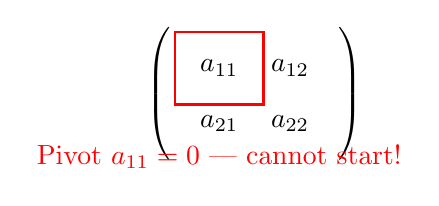
\begin{tikzpicture}[scale=0.7]
\matrix (m) [matrix of math nodes, left delimiter=(, right delimiter=),
             nodes={minimum width=0.9cm, minimum height=0.7cm}] {
  a_{11} & a_{12} \\
  a_{21} & a_{22} \\
};
\node[draw=red, thick, fit=(m-1-1), inner sep=3pt] {};
\node[below=0.5cm of m-1-1, red] {Pivot $a_{11} = 0$ — cannot start!};
\end{tikzpicture}
\end{center}

Even later pivots can fail:
$$\begin{pmatrix} 1 & 2 & 3 \\ 1 & 2 & 4 \\ 1 & 3 & 5 \end{pmatrix}
\xrightarrow{\text{after } R_1} \begin{pmatrix}
\rem{0} & \rem{0} & \rem{0} \\
\rem{0} & \pvt{0} & 1 \\
\rem{0} & 1 & 2
\end{pmatrix}$$

Second pivot is $\pvt{0}$!

\vspace{0.2cm}
\textbf{Solution}: Permute rows first (swap to get nonzero pivot) $\to$ \x{PLU decomposition} (Week 3).
\end{frame}

% ═══════════════════════════════════════
% §7 SUMMARY
% ═══════════════════════════════════════
\section{Summary}

\begin{frame}{Summary}
\textbf{Today we learned:}

\begin{enumerate}
\item \textbf{Rank-one matrix}: $R = \mathbf{u}\,\mathbf{v}^T$ (one pattern, repeated)

\item \textbf{Cross-filling algorithm}: Decompose any matrix into rank-one pieces
$$A = R_1 + R_2 + \cdots + R_r$$
Pick pivot $\to$ Extract cross $\to$ Fill $\to$ Subtract $\to$ Repeat

\item \textbf{Pivot selection principle}: Choose any nonzero entry in the remaindering matrix $\to$ flexible decompositions

\item \textbf{Pivot flexibility}: Different pivot sequences $\to$ different decompositions, same rank

\item \textbf{Sum $\leftrightarrow$ Product equivalence}:
$$\sum_{k=1}^r \mathbf{u}_k\,\mathbf{v}_k^T = A = UV$$

\item \textbf{Rank} = number of pieces = inner dimension of $UV$

\item \textbf{Special case}: Diagonal pivots $\to$ LU decomposition
\end{enumerate}
\end{frame}

\begin{frame}{Looking Ahead}
\textbf{Lecture 4} (next week):
\begin{itemize}
\item \x{Well-definedness of rank} — Why does rank not depend on pivot choices?
\item \x{Linear independence} and \x{basis} — Two languages for subspaces
\item \x{Dimension} — Connection to rank via trace
\item Solving $Ax = b$ using cross-filling
\end{itemize}

\vfill
\textbf{The big picture}:
\begin{center}
Cross-filling $\to$ Rank $\to$ Subspaces $\to$ Projections $\to$ Spectral Decomposition
\end{center}

Every major topic connects back to rank-one decomposition!
\end{frame}

\end{document}
